
\section{Bonus}
\label{sec:Bonus}

So far, we’ve worked with audio embeddings, that were created from a pre-trained and frozen sound event detection model. 
To receive the bonus points, train one of our pre-trained sound event detection models on the MLPC dataset to predict the ten sound categories of interest in an end-to-end manner. 
You can find an implementation, a detailed documentation and pre-trained checkpoints here: \url{https://github.com/fschmid56/PretrainedSED} . 
Use one of the checkpoint that was pre-trained on AudioSet-strong as a starting point. 
You can use any of the model architectures. 
Compare the performance of the resulting system to the best model from the previous section.



\subsection{Train one of our pre-trained sound event detection models on the MLPC dataset to predict the ten sound categories of interest in an end-to-end manner.}
\label{sec:Bonus:a}

\begin{figure}[htbp]
    \centering
    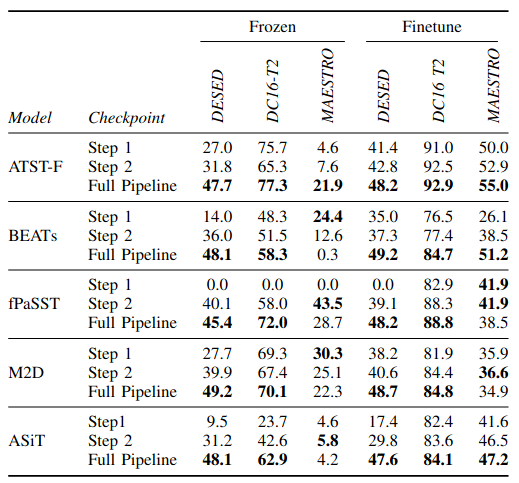
\includegraphics[width=0.4\textwidth]{figs/downstream_task_results.png}
    \caption{Downstream Task Performances}
    \label{fig:Downstream Task Performances}
\end{figure}



\subsection{You can use any of the model architectures.}
\label{sec:Bonus:b}

We wanted to use a Transformer model as we haven't tested it yet. Due to the downstream task performance (Figure~\ref{fig:Downstream Task Performances}), we decided on the model ATST-F (./models/atstframe).
\newline
We used the Pre-Trained Model Checkpoint from here: 
\newline

\url{https://github.com/fschmid56/PretrainedSED/releases/download/v0.0.1/ATST-F_strong_1.pt} .



\subsection{Compare the performance of the resulting system to the best model from the previous section.}
\label{sec:Bonus:c}




